\documentclass[tikz,border=10pt]{standalone}
\begin{document}
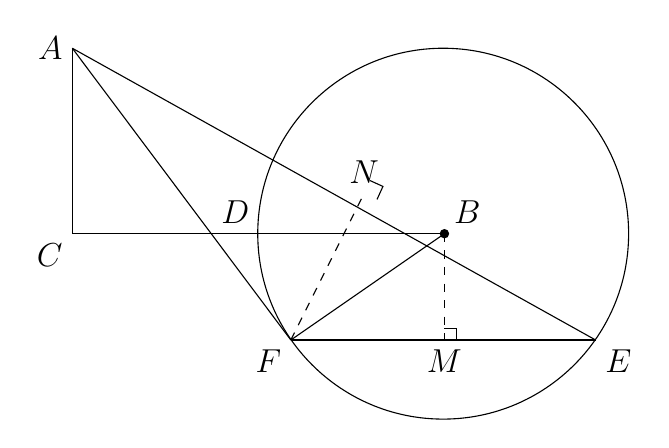
\begin{tikzpicture}[scale=1.5, font=\large]
  % Points
  \coordinate (A) at (0.78,-0.57);
  \coordinate (C) at (0.78,-2.14);
  \coordinate (D) at (1.96,-2.14);
  \coordinate (B) at (3.93,-2.14);
  \coordinate (F) at (2.63,-3.04);
  \coordinate (E) at (5.21,-3.04);
  \coordinate (M) at (3.93,-3.04);
  \coordinate (N) at (3.25,-1.80);

  % Circle
  \draw (3.92,-2.14) circle (1.57);

  % Solid edges
  \draw (A) -- (C);
  \draw (C) -- (B);
  \draw (A) -- (E);
  \draw (A) -- (F);
  \draw (F) -- (B);
  \draw (F) -- (E);

  % Dashed edges
  \draw[dashed] (F) -- (N);
  \draw[dashed] (B) -- (M);

  % Right-angle marks
  \draw (3.93,-2.94) -- (4.03,-2.94) -- (4.03,-3.04);
  \draw (3.36,-1.85) -- (3.41,-1.74) -- (3.30,-1.69);

  % Points
  \fill (B) circle (0.04);

  % Labels
  \node[left] at (A) {$A$};
  \node[below left] at (C) {$C$};
  \node[above right] at (D) {$D$};
  \node[above right] at (B) {$B$};
  \node[above] at (N) {$N$};
  \node[below left] at (F) {$F$};
  \node[below] at (M) {$M$};
  \node[below right] at (E) {$E$};
\end{tikzpicture}
\end{document}
